\documentclass[twoside]{book}

% Packages required by doxygen
\usepackage{fixltx2e}
\usepackage{calc}
\usepackage{doxygen}
\usepackage{graphicx}
\usepackage[utf8]{inputenc}
\usepackage{makeidx}
\usepackage{multicol}
\usepackage{multirow}
\PassOptionsToPackage{warn}{textcomp}
\usepackage{textcomp}
\usepackage[nointegrals]{wasysym}
\usepackage[table]{xcolor}

% Font selection
\usepackage[T1]{fontenc}
\usepackage{mathptmx}
\usepackage[scaled=.90]{helvet}
\usepackage{courier}
\usepackage{amssymb}
\usepackage{sectsty}
\renewcommand{\familydefault}{\sfdefault}
\allsectionsfont{%
  \fontseries{bc}\selectfont%
  \color{darkgray}%
}
\renewcommand{\DoxyLabelFont}{%
  \fontseries{bc}\selectfont%
  \color{darkgray}%
}
\newcommand{\+}{\discretionary{\mbox{\scriptsize$\hookleftarrow$}}{}{}}

% Page & text layout
\usepackage{geometry}
\geometry{%
  a4paper,%
  top=2.5cm,%
  bottom=2.5cm,%
  left=2.5cm,%
  right=2.5cm%
}
\tolerance=750
\hfuzz=15pt
\hbadness=750
\setlength{\emergencystretch}{15pt}
\setlength{\parindent}{0cm}
\setlength{\parskip}{0.2cm}
\makeatletter
\renewcommand{\paragraph}{%
  \@startsection{paragraph}{4}{0ex}{-1.0ex}{1.0ex}{%
    \normalfont\normalsize\bfseries\SS@parafont%
  }%
}
\renewcommand{\subparagraph}{%
  \@startsection{subparagraph}{5}{0ex}{-1.0ex}{1.0ex}{%
    \normalfont\normalsize\bfseries\SS@subparafont%
  }%
}
\makeatother

% Headers & footers
\usepackage{fancyhdr}
\pagestyle{fancyplain}
\fancyhead[LE]{\fancyplain{}{\bfseries\thepage}}
\fancyhead[CE]{\fancyplain{}{}}
\fancyhead[RE]{\fancyplain{}{\bfseries\leftmark}}
\fancyhead[LO]{\fancyplain{}{\bfseries\rightmark}}
\fancyhead[CO]{\fancyplain{}{}}
\fancyhead[RO]{\fancyplain{}{\bfseries\thepage}}
\fancyfoot[LE]{\fancyplain{}{}}
\fancyfoot[CE]{\fancyplain{}{}}
\fancyfoot[RE]{\fancyplain{}{\bfseries\scriptsize Generated on Tue Nov 4 2014 12\+:16\+:45 for segmentation by Doxygen }}
\fancyfoot[LO]{\fancyplain{}{\bfseries\scriptsize Generated on Tue Nov 4 2014 12\+:16\+:45 for segmentation by Doxygen }}
\fancyfoot[CO]{\fancyplain{}{}}
\fancyfoot[RO]{\fancyplain{}{}}
\renewcommand{\footrulewidth}{0.4pt}
\renewcommand{\chaptermark}[1]{%
  \markboth{#1}{}%
}
\renewcommand{\sectionmark}[1]{%
  \markright{\thesection\ #1}%
}

% Indices & bibliography
\usepackage{natbib}
\usepackage[titles]{tocloft}
\setcounter{tocdepth}{3}
\setcounter{secnumdepth}{5}
\makeindex

% Hyperlinks (required, but should be loaded last)
\usepackage{ifpdf}
\ifpdf
  \usepackage[pdftex,pagebackref=true]{hyperref}
\else
  \usepackage[ps2pdf,pagebackref=true]{hyperref}
\fi
\hypersetup{%
  colorlinks=true,%
  linkcolor=blue,%
  citecolor=blue,%
  unicode%
}

% Custom commands
\newcommand{\clearemptydoublepage}{%
  \newpage{\pagestyle{empty}\cleardoublepage}%
}


%===== C O N T E N T S =====

\begin{document}

% Titlepage & ToC
\pagenumbering{roman}
\begin{titlepage}
\vspace*{7cm}
\begin{center}%
{\Large segmentation }\\
\vspace*{1cm}
{\large Generated by Doxygen 1.8.8}\\
\vspace*{0.5cm}
{\small Tue Nov 4 2014 12:16:45}\\
\end{center}
\end{titlepage}
\clearemptydoublepage
\tableofcontents
\clearemptydoublepage
\pagenumbering{arabic}

%--- Begin generated contents ---
\chapter{Module Index}
\section{Modules}
Here is a list of all modules\+:\begin{DoxyCompactList}
\item \contentsline{section}{edison\+Segmentation}{\pageref{group__icub__edisonSegmentation}}{}
\item \contentsline{section}{graphbased\+Segmentation}{\pageref{group__icub__graphbasedSegmentation}}{}
\end{DoxyCompactList}

\chapter{Hierarchical Index}
\section{Class Hierarchy}
This inheritance list is sorted roughly, but not completely, alphabetically\+:\begin{DoxyCompactList}
\item \contentsline{section}{Edison\+Segm\+Module}{\pageref{classEdisonSegmModule}}{}
\item \contentsline{section}{yarp\+:\+:sig\+:\+:Pixel}{\pageref{classyarp_1_1sig_1_1Pixel}}{}
\item \contentsline{section}{yarp\+:\+:sig\+:\+:Segmentation\+Module\+Interface}{\pageref{classyarp_1_1sig_1_1SegmentationModuleInterface}}{}
\begin{DoxyCompactList}
\item \contentsline{section}{G\+B\+Segm\+Module}{\pageref{classGBSegmModule}}{}
\end{DoxyCompactList}
\end{DoxyCompactList}

\chapter{Data Structure Index}
\section{Data Structures}
Here are the data structures with brief descriptions\+:\begin{DoxyCompactList}
\item\contentsline{section}{\hyperlink{classEdisonSegmModule}{Edison\+Segm\+Module} \\*Edison Segmentation Module }{\pageref{classEdisonSegmModule}}{}
\item\contentsline{section}{\hyperlink{classGBSegmModule}{G\+B\+Segm\+Module} \\*Segmentation Module }{\pageref{classGBSegmModule}}{}
\item\contentsline{section}{\hyperlink{classyarp_1_1sig_1_1Pixel}{yarp\+::sig\+::\+Pixel} \\*\hyperlink{classyarp_1_1sig_1_1Pixel}{Pixel} position in the image frame }{\pageref{classyarp_1_1sig_1_1Pixel}}{}
\item\contentsline{section}{\hyperlink{classyarp_1_1sig_1_1SegmentationModuleInterface}{yarp\+::sig\+::\+Segmentation\+Module\+Interface} \\*Interface for module that performs graph-\/based segmentation }{\pageref{classyarp_1_1sig_1_1SegmentationModuleInterface}}{}
\end{DoxyCompactList}

\chapter{Module Documentation}
\section{edison\+Segmentation}
\label{group__icub__edisonSegmentation}\index{edison\+Segmentation@{edison\+Segmentation}}


Wrapper to the The E\+D\+I\+S\+O\+N system\+: a low-\/level vision tool that performs confidence based edge detection and synergistic image segmentation.  


Wrapper to the The E\+D\+I\+S\+O\+N system\+: a low-\/level vision tool that performs confidence based edge detection and synergistic image segmentation. 

\hypertarget{group__icub__graphbasedSegmentation_intro_sec}{}\subsection{Description}\label{group__icub__graphbasedSegmentation_intro_sec}
This module wraps around some functions of the E\+D\+I\+S\+O\+N system from the robust image understanding laboratory at Rutgers University.

The purpose of the module is to obtain good segmentation of color images. The image is split into regions corresponding to uniformly colored patches.

Details on the employed algorithms is provided in the following paper\+: \mbox{[}1\mbox{]} D. Comaniciu, P. Meer\+: \char`\"{}\+Mean shift\+: A robust approach toward feature space analysis\char`\"{}. I\+E\+E\+E Trans. Pattern Anal. Machine Intell., May 2002.

\mbox{[}2\mbox{]} P. Meer, B. Georgescu\+: \char`\"{}\+Edge detection with embedded confidence\char`\"{}. I\+E\+E\+E Trans. Pattern Anal. Machine Intell., 28, 2001.

\mbox{[}3\mbox{]} C. Christoudias, B. Georgescu, P. Meer\+: \char`\"{}\+Synergism in low level vision\char`\"{}. 16th International Conference of Pattern Recognition, Track 1 -\/ Computer Vision and Robotics, Quebec City, Canada, August 2001.

The edison source files are provided as a library in the edisonlib folder.

Some changes to these files had to be made in order to obtain the desired functionality. These include changes in function Get\+Regions in \hyperlink{msImageProcessor_8cpp_source}{ms\+Image\+Processor.\+cpp}\hypertarget{group__icub__graphbasedSegmentation_lib_sec}{}\subsection{Libraries}\label{group__icub__graphbasedSegmentation_lib_sec}
Y\+A\+R\+P library Open\+C\+V library\hypertarget{group__icub__graphbasedSegmentation_parameters_sec}{}\subsection{Parameters}\label{group__icub__graphbasedSegmentation_parameters_sec}
width, height -\/ Dimension of the images to be processed. This may differ from the dimension of the input images. Forcing a smaller dimension will save computation power at the cost of resolution. Values larger that the input image dimension will be discarded. These parameters do no influence the dimension of the output. This is always the same as the input dimension. Default\+: the size of the original image.

sigma\+S -\/ The spatial bandwidth (neighborhood in the pixel domain). Default\+: 7

sigma\+R -\/ The color bandwidth (neighborhood in the color color domain). Default\+: 6.\+5

minregion -\/ The minimal area for segmented regions (in pixels) Default\+: 20.\+0

grad\+Win\+Rad -\/ The radius of the window used for the computation of the gradient and confidence map (positive integer). Default\+: 2.\+0

threshold -\/ edge strength threshold (must be in the interval \mbox{[}0,1\mbox{]}) Default\+: 0.\+3

mixture -\/ mixture parameter (must be in the interval \mbox{[}0,1\mbox{]}) Default\+: 0.\+2

speedup -\/ accelerate computation by doing some approximations. Possible values 0 (N\+O\+\_\+\+S\+P\+E\+E\+D\+U\+P), 1 (M\+E\+D\+\_\+\+S\+P\+E\+E\+D\+U\+P), 2 (H\+I\+G\+H\+\_\+\+S\+P\+E\+E\+D\+U\+P) Default\+: M\+E\+D\+\_\+\+S\+P\+E\+E\+D\+U\+P

The best results have been obtained with M\+E\+D\+\_\+\+S\+P\+E\+E\+D\+U\+P\hypertarget{group__icub__graphbasedSegmentation_portsa_sec}{}\subsection{Ports Accessed}\label{group__icub__graphbasedSegmentation_portsa_sec}
Port with raw R\+G\+B image.\hypertarget{group__icub__graphbasedSegmentation_portsc_sec}{}\subsection{Ports Created}\label{group__icub__graphbasedSegmentation_portsc_sec}
/conf for module configuration, according to E\+D\+I\+S\+O\+Nsegmentation.\+thrift definition file

/raw\+Img\+:i receive the original R\+G\+B image to segment

/raw\+Img\+:o output the original R\+G\+B image

/labeled\+Img\+:o segmented image with the labels (Pixel\+Int)

/view\+Img\+:o segmented image with the colors models for each region (good to visualize)\hypertarget{group__icub__graphbasedSegmentation_in_files_sec}{}\subsection{Input Data Files}\label{group__icub__graphbasedSegmentation_in_files_sec}
None\hypertarget{group__icub__graphbasedSegmentation_out_data_sec}{}\subsection{Output Data Files}\label{group__icub__graphbasedSegmentation_out_data_sec}
None\hypertarget{group__icub__graphbasedSegmentation_conf_file_sec}{}\subsection{Configuration Files}\label{group__icub__graphbasedSegmentation_conf_file_sec}
Parameters can be put in a configuration file. Default configuration file name is edison\+Config.\+ini An example configuration file is provided in the source folder (config\+File.\+ini), containing the following\+: 
\begin{DoxyCode}
height 120
width 160
dim 3
sigmaS 10       
sigmaR 18       
minRegion 50  
gradWindRad  2 
threshold  1 
mixture  1  
speedup 1
\end{DoxyCode}
\hypertarget{group__icub__graphbasedSegmentation_tested_os_sec}{}\subsection{Tested O\+S}\label{group__icub__graphbasedSegmentation_tested_os_sec}
Linux and Windows.\hypertarget{group__icub__graphbasedSegmentation_example_sec}{}\subsection{Example Instantiation of the Module}\label{group__icub__graphbasedSegmentation_example_sec}

\begin{DoxyCode}
yarp server
edisonSegmentation.exe --from configFile.ini
yarpdev --device opencv\_grabber --movie H:\(\backslash\)DataSets\(\backslash\)testImages2009\_07\_21\(\backslash\)segm\_test\_icub.avi --loop --
      framerate 0.1
yarpview /raw
yarpview /view
yarp connect /grabber /edisonSegm/rawImg:i
yarp connect /edisonSegm/rawImg:o /raw
yarp connect /edisonSegm/viewImg:o /view
\end{DoxyCode}


\begin{DoxyAuthor}{Author}
Alexandre Bernardino, Elena Ceseracciu (improved module version)
\end{DoxyAuthor}
Copyright (C) 2008 Robot\+Cub Consortium

Copy\+Policy\+: Released under the terms of the G\+N\+U G\+P\+L v2.\+0.

This file can be edited at src/edison\+Segmentation/main.\+cpp. 
\section{graphbased\+Segmentation}
\label{group__icub__graphbasedSegmentation}\index{graphbased\+Segmentation@{graphbased\+Segmentation}}


Wrapper module that performs graph-\/based image segmentation exploiting the algorithm developed by Felzenszwalb and Huttenlocher (Brown University).  


Wrapper module that performs graph-\/based image segmentation exploiting the algorithm developed by Felzenszwalb and Huttenlocher (Brown University). 

\hypertarget{group__icub__graphbasedSegmentation_intro_sec}{}\subsection{Description}\label{group__icub__graphbasedSegmentation_intro_sec}
Wrapper module that performs graph-\/based image segmentation exploiting the algorithm developed by Felzenszwalb and Huttenlocher (Brown University). The algorithm is described in the paper \char`\"{}\+Efficient Graph-\/\+Based Image Segmentation\char`\"{}, Pedro F. Felzenszwalb and Daniel P. Huttenlocher, International Journal of Computer Vision, Volume 59, Number 2, September 2004. The original code is available from \href{http://www.cs.brown.edu/~pff/segment/}{\tt http\+://www.\+cs.\+brown.\+edu/$\sim$pff/segment/} and has been copied into the src/segmentation/graph\+Based/segment folder.\hypertarget{group__icub__graphbasedSegmentation_lib_sec}{}\subsection{Libraries}\label{group__icub__graphbasedSegmentation_lib_sec}
Y\+A\+R\+P library.\hypertarget{group__icub__graphbasedSegmentation_parameters_sec}{}\subsection{Parameters}\label{group__icub__graphbasedSegmentation_parameters_sec}

\begin{DoxyItemize}
\item {\ttfamily name} name of the module (for opened ports)
\item {\ttfamily sigma} smoothing parameter (standard deviation of a Gaussian filter used to pre-\/process image, in order to compensate for digitization artifacts)
\item {\ttfamily k} scale factor for boundary-\/detection threshold function (a larger k causes a preference for larger components).
\item {\ttfamily min\+Region} minumum size of a component.
\end{DoxyItemize}\hypertarget{group__icub__graphbasedSegmentation_portsa_sec}{}\subsection{Ports Accessed}\label{group__icub__graphbasedSegmentation_portsa_sec}
None.\hypertarget{group__icub__graphbasedSegmentation_portsc_sec}{}\subsection{Ports Created}\label{group__icub__graphbasedSegmentation_portsc_sec}

\begin{DoxyItemize}
\item /$<$module\+\_\+name$>$/raw\+Img\+:i input port where original images must be sent (default\+: G\+B\+Seg)
\item /$<$module\+\_\+name$>$/view\+Img\+:o
\item /$<$module\+\_\+name$>$/conf rpc port, accepts the commands defined in \hyperlink{}{graph\+Based\+Segmentation\+Interface.\+thrift } and documented \hyperlink{}{here }
\end{DoxyItemize}\hypertarget{group__icub__graphbasedSegmentation_in_files_sec}{}\subsection{Input Data Files}\label{group__icub__graphbasedSegmentation_in_files_sec}
None\hypertarget{group__icub__graphbasedSegmentation_out_data_sec}{}\subsection{Output Data Files}\label{group__icub__graphbasedSegmentation_out_data_sec}
None\hypertarget{group__icub__graphbasedSegmentation_conf_file_sec}{}\subsection{Configuration Files}\label{group__icub__graphbasedSegmentation_conf_file_sec}
No configuration file is needed. Parameters described in \hyperlink{group__icub__graphbasedSegmentation_parameters_sec}{Parameters} can be provided in a configuration file; default filename is\hypertarget{group__icub__graphbasedSegmentation_tested_os_sec}{}\subsection{Tested O\+S}\label{group__icub__graphbasedSegmentation_tested_os_sec}
Linux and Windows.\hypertarget{group__icub__graphbasedSegmentation_example_sec}{}\subsection{Example Instantiation of the Module}\label{group__icub__graphbasedSegmentation_example_sec}
Examples of module use are provided in the app/scripts folder, and installed into app/graph\+Based\+Segm/scripts.

\begin{DoxyAuthor}{Author}
Elena Ceseracciu
\end{DoxyAuthor}
Copyright (C) 2012 R\+B\+C\+S -\/ Istituto Italiano di Tecnologia

Copy\+Policy\+: Released under the terms of the G\+N\+U G\+P\+L v2.\+0 and later.

This file can be edited at src/segmentation/graph\+Based/main.\+cpp. 
\chapter{Data Structure Documentation}
\section{Edison\+Segm\+Module Class Reference}
\label{classEdisonSegmModule}\index{Edison\+Segm\+Module@{Edison\+Segm\+Module}}


Edison Segmentation Module.  




{\ttfamily \#include $<$Edison\+Segm\+Module.\+h$>$}



Inherits R\+F\+Module, and Segmentation\+Module.

\subsection*{Public Member Functions}
\begin{DoxyCompactItemize}
\item 
virtual bool {\bfseries configure} (yarp\+::os\+::\+Resource\+Finder \&rf)\label{classEdisonSegmModule_adff5acfcb2411234172937f50071f747}

\item 
virtual bool {\bfseries close} ()\label{classEdisonSegmModule_a01831b02110aa3c2dfb2ae2a235f32c8}

\item 
virtual bool {\bfseries interrupt\+Module} ()\label{classEdisonSegmModule_a050c4fd290134b2c549f1f255b39e3fa}

\item 
virtual bool {\bfseries update\+Module} ()\label{classEdisonSegmModule_a9ec945c0f1cd4246d94255c9d58bbd4f}

\item 
bool {\bfseries attach} (yarp\+::os\+::\+Port \&source)\label{classEdisonSegmModule_a1ac9b550e805a1e1dff863205b70e553}

\item 
virtual void {\bfseries set\+\_\+sigma\+S} (const double new\+Value)\label{classEdisonSegmModule_a9331b900b7671ad851f9aa3b4159e0cf}

\item 
virtual void {\bfseries set\+\_\+sigma\+R} (const double new\+Value)\label{classEdisonSegmModule_a26d36ebd0382e29033d6b4764b1cfb33}

\item 
virtual void {\bfseries set\+\_\+min\+Region} (const double new\+Value)\label{classEdisonSegmModule_a9f4a7a594ff5ee50d330cb964dd9b48f}

\item 
virtual void {\bfseries set\+\_\+grad\+Wind\+Rad} (const double new\+Value)\label{classEdisonSegmModule_a6add88774ea4794f278988a44d4a64c2}

\item 
virtual void {\bfseries set\+\_\+threshold} (const double new\+Value)\label{classEdisonSegmModule_a63a8a762fcad79343218570b175b755d}

\item 
virtual void {\bfseries set\+\_\+mixture} (const double new\+Value)\label{classEdisonSegmModule_a0993cc82cbd9dfb774e69e40a236787a}

\item 
virtual void {\bfseries set\+\_\+speedup} (const Speed\+Up\+Level\+Comm new\+Speed\+Level)\label{classEdisonSegmModule_af35d584ee6446611e1c483897c86f1fc}

\item 
virtual double {\bfseries get\+\_\+sigma\+S} ()\label{classEdisonSegmModule_a62aa5009cad7d09959ed5cdd8c358a90}

\item 
virtual double {\bfseries get\+\_\+sigma\+R} ()\label{classEdisonSegmModule_ad1045be0e10cd0d40c81396f48e54b9a}

\item 
virtual double {\bfseries get\+\_\+min\+Region} ()\label{classEdisonSegmModule_ad61a5ccea53f415be9f2b76a8781689f}

\item 
virtual double {\bfseries get\+\_\+grad\+Wind\+Rad} ()\label{classEdisonSegmModule_ab9ce5f24dd33f58d543b25ec0257af41}

\item 
virtual double {\bfseries get\+\_\+threshold} ()\label{classEdisonSegmModule_a8e3ab7941df516f42357330a80d1e408}

\item 
virtual double {\bfseries get\+\_\+mixture} ()\label{classEdisonSegmModule_a58df44d5dbba062170e5e22f957da907}

\item 
virtual Speed\+Up\+Level\+Comm {\bfseries get\+\_\+speedup} ()\label{classEdisonSegmModule_ae1f22b6113534640a3faedd22505932b}

\item 
virtual bool {\bfseries read} (yarp\+::os\+::\+Connection\+Reader \&connection)\label{classSegmentationModule_a99d3baa0d96cb5a8a7aeef226759ef73}

\end{DoxyCompactItemize}


\subsection{Detailed Description}
Edison Segmentation Module. 



Definition at line 35 of file Edison\+Segm\+Module.\+h.



The documentation for this class was generated from the following files\+:\begin{DoxyCompactItemize}
\item 
C\+:/dev/icub-\/contrib-\/iit/segmentation/\+E\+D\+I\+S\+O\+N/Edison\+Segm\+Module.\+h\item 
C\+:/dev/icub-\/contrib-\/iit/segmentation/\+E\+D\+I\+S\+O\+N/Edison\+Segm\+Module.\+cpp\end{DoxyCompactItemize}

\section{G\+B\+Segm\+Module Class Reference}
\label{classGBSegmModule}\index{G\+B\+Segm\+Module@{G\+B\+Segm\+Module}}


Segmentation Module.  




{\ttfamily \#include $<$Segm\+Module.\+h$>$}

Inheritance diagram for G\+B\+Segm\+Module\+:\begin{figure}[H]
\begin{center}
\leavevmode
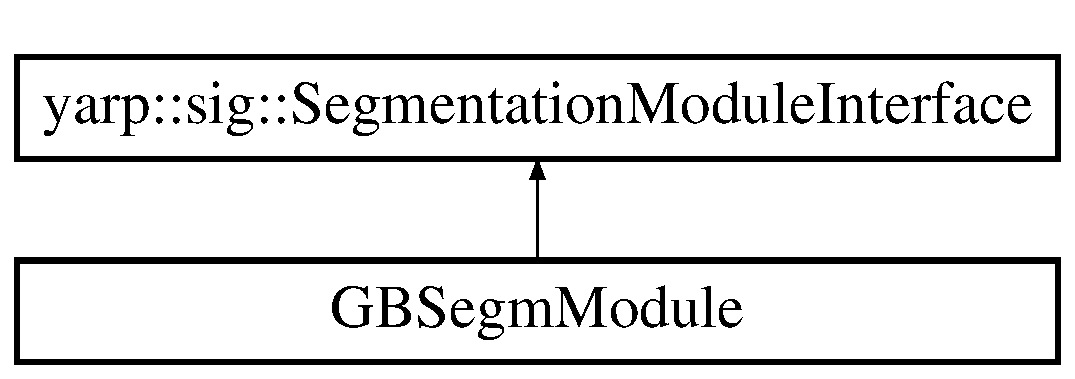
\includegraphics[height=2.000000cm]{classGBSegmModule}
\end{center}
\end{figure}
\subsection*{Public Member Functions}
\begin{DoxyCompactItemize}
\item 
virtual bool {\bfseries configure} (yarp\+::os\+::\+Resource\+Finder \&rf)\label{classGBSegmModule_ada22cbfc66dd9b75a7a824e1ce642639}

\item 
virtual bool {\bfseries close} ()\label{classGBSegmModule_ac3259b29883674bf47aa962f54806913}

\item 
virtual bool {\bfseries interrupt\+Module} ()\label{classGBSegmModule_a99b9908ade3135dd5ee491b799d5e171}

\item 
virtual bool {\bfseries update\+Module} ()\label{classGBSegmModule_a66f40b6ae480a039a2c10f6b91c59dde}

\item 
bool {\bfseries attach} (yarp\+::os\+::\+Port \&source)\label{classGBSegmModule_a4ae8d5fee391d799299a10e09a5ea8c4}

\item 
virtual void \hyperlink{classGBSegmModule_a27ffe08d394d321d9f9441423d36ef5e}{set\+\_\+sigma} (const double new\+Value)
\begin{DoxyCompactList}\small\item\em Set sigma (smoothing) parameter for the algorithm. \end{DoxyCompactList}\item 
virtual void \hyperlink{classGBSegmModule_a15129913273e221a46c428f697e40575}{set\+\_\+k} (const double new\+Value)
\begin{DoxyCompactList}\small\item\em Set k (scale factor for boundary-\/detection threshold function) parameter for the algorithm. \end{DoxyCompactList}\item 
virtual void \hyperlink{classGBSegmModule_ae1c722c9c774cbde4f6bfada3f0826ba}{set\+\_\+min\+Region} (const double new\+Value)
\begin{DoxyCompactList}\small\item\em Set min\+Region parameter for the algorithm, i.\+e., the minimum size of any segmented component. \end{DoxyCompactList}\item 
virtual double \hyperlink{classGBSegmModule_ae32ae1b1461e19c3a1b2f429c729ed03}{get\+\_\+sigma} ()
\begin{DoxyCompactList}\small\item\em Get sigma (smoothing) parameter for the algorithm. \end{DoxyCompactList}\item 
virtual double \hyperlink{classGBSegmModule_a44bab99aa7a035e57a185673c040d2f6}{get\+\_\+k} ()
\begin{DoxyCompactList}\small\item\em Get k (scale factor for boundary-\/detection threshold function) parameter for the algorithm. \end{DoxyCompactList}\item 
virtual double \hyperlink{classGBSegmModule_a2378b95e60b406a119947aa86b5bb9c4}{get\+\_\+min\+Region} ()
\begin{DoxyCompactList}\small\item\em Get min\+Region parameter for the algorithm, i.\+e., the minimum size of any segmented component. \end{DoxyCompactList}\item 
virtual int32\+\_\+t \hyperlink{classGBSegmModule_a655ee7c895eed07b07099133b9d8ce68}{get\+\_\+num\+\_\+components} ()
\begin{DoxyCompactList}\small\item\em Get the number of segmented components that have been detected in the last provided image. \end{DoxyCompactList}\item 
virtual std\+::vector\\*
$<$ \hyperlink{classyarp_1_1sig_1_1Pixel}{yarp\+::sig\+::\+Pixel} $>$ \hyperlink{classGBSegmModule_a0b63c53513e67c4f126e29cf7f28ad53}{get\+\_\+component\+\_\+around} (const \hyperlink{classyarp_1_1sig_1_1Pixel}{yarp\+::sig\+::\+Pixel} \&obj\+Center)
\begin{DoxyCompactList}\small\item\em Get the list of pixels corresponding to the component to which a given pixel belongs. \end{DoxyCompactList}\item 
virtual bool {\bfseries read} (yarp\+::os\+::\+Connection\+Reader \&connection)\label{classyarp_1_1sig_1_1SegmentationModuleInterface_ae35adf3fde4e4dd6e2dea92b6e396794}

\end{DoxyCompactItemize}


\subsection{Detailed Description}
Segmentation Module. 



Definition at line 37 of file Segm\+Module.\+h.



\subsection{Member Function Documentation}
\index{G\+B\+Segm\+Module@{G\+B\+Segm\+Module}!get\+\_\+component\+\_\+around@{get\+\_\+component\+\_\+around}}
\index{get\+\_\+component\+\_\+around@{get\+\_\+component\+\_\+around}!G\+B\+Segm\+Module@{G\+B\+Segm\+Module}}
\subsubsection[{get\+\_\+component\+\_\+around}]{\setlength{\rightskip}{0pt plus 5cm}std\+::vector$<$ {\bf Pixel} $>$ G\+B\+Segm\+Module\+::get\+\_\+component\+\_\+around (
\begin{DoxyParamCaption}
\item[{const {\bf yarp\+::sig\+::\+Pixel} \&}]{obj\+Center}
\end{DoxyParamCaption}
)\hspace{0.3cm}{\ttfamily [virtual]}}\label{classGBSegmModule_a0b63c53513e67c4f126e29cf7f28ad53}


Get the list of pixels corresponding to the component to which a given pixel belongs. 


\begin{DoxyParams}{Parameters}
{\em obj\+Center} & a pixel belonging to the region of interest \\
\hline
\end{DoxyParams}
\begin{DoxyReturn}{Returns}
list of pixels belonging to the same component as the input pixels 
\end{DoxyReturn}


Reimplemented from \hyperlink{classyarp_1_1sig_1_1SegmentationModuleInterface_a9bf0b95fbab216b2284122b0b8a36820}{yarp\+::sig\+::\+Segmentation\+Module\+Interface}.



Definition at line 72 of file Segm\+Module.\+cpp.



References yarp\+::sig\+::\+Pixel\+::x, and yarp\+::sig\+::\+Pixel\+::y.


\begin{DoxyCode}
73 \{
74     vector<Pixel> result;
75     result.clear();
76     segMutex.wait();
77     rgb componentColor = imRef(seg, objCenter.x, objCenter.y);
78     \textcolor{keywordflow}{for} (\textcolor{keywordtype}{int} y = 0; y < seg->height(); y++) \{
79 
80             \textcolor{keywordflow}{for} (\textcolor{keywordtype}{int} x = 0; x < seg->width(); x++) \{
81 
82               \textcolor{keywordflow}{if} (imRef(seg, x, y) == componentColor)
83                 result.push\_back(Pixel(x, y));
84 
85 
86             \}
87 
88         \}
89 
90     
91     segMutex.post();
92     \textcolor{keywordflow}{return} result;
93 
94 \}
\end{DoxyCode}
\index{G\+B\+Segm\+Module@{G\+B\+Segm\+Module}!get\+\_\+k@{get\+\_\+k}}
\index{get\+\_\+k@{get\+\_\+k}!G\+B\+Segm\+Module@{G\+B\+Segm\+Module}}
\subsubsection[{get\+\_\+k}]{\setlength{\rightskip}{0pt plus 5cm}double G\+B\+Segm\+Module\+::get\+\_\+k (
\begin{DoxyParamCaption}
{}
\end{DoxyParamCaption}
)\hspace{0.3cm}{\ttfamily [virtual]}}\label{classGBSegmModule_a44bab99aa7a035e57a185673c040d2f6}


Get k (scale factor for boundary-\/detection threshold function) parameter for the algorithm. 

\begin{DoxyReturn}{Returns}
current value for k parameter 
\end{DoxyReturn}


Reimplemented from \hyperlink{classyarp_1_1sig_1_1SegmentationModuleInterface_a91f3d872a48599337d1d2f365ac4c31e}{yarp\+::sig\+::\+Segmentation\+Module\+Interface}.



Definition at line 69 of file Segm\+Module.\+cpp.


\begin{DoxyCode}
69 \{\textcolor{keywordflow}{return} k;\}
\end{DoxyCode}
\index{G\+B\+Segm\+Module@{G\+B\+Segm\+Module}!get\+\_\+min\+Region@{get\+\_\+min\+Region}}
\index{get\+\_\+min\+Region@{get\+\_\+min\+Region}!G\+B\+Segm\+Module@{G\+B\+Segm\+Module}}
\subsubsection[{get\+\_\+min\+Region}]{\setlength{\rightskip}{0pt plus 5cm}double G\+B\+Segm\+Module\+::get\+\_\+min\+Region (
\begin{DoxyParamCaption}
{}
\end{DoxyParamCaption}
)\hspace{0.3cm}{\ttfamily [virtual]}}\label{classGBSegmModule_a2378b95e60b406a119947aa86b5bb9c4}


Get min\+Region parameter for the algorithm, i.\+e., the minimum size of any segmented component. 

\begin{DoxyReturn}{Returns}
current value for min\+Region parameter 
\end{DoxyReturn}


Reimplemented from \hyperlink{classyarp_1_1sig_1_1SegmentationModuleInterface_a6c184aeea894f6afcc342c5aa748429d}{yarp\+::sig\+::\+Segmentation\+Module\+Interface}.



Definition at line 70 of file Segm\+Module.\+cpp.


\begin{DoxyCode}
70 \{\textcolor{keywordflow}{return} min\_size;\}
\end{DoxyCode}
\index{G\+B\+Segm\+Module@{G\+B\+Segm\+Module}!get\+\_\+num\+\_\+components@{get\+\_\+num\+\_\+components}}
\index{get\+\_\+num\+\_\+components@{get\+\_\+num\+\_\+components}!G\+B\+Segm\+Module@{G\+B\+Segm\+Module}}
\subsubsection[{get\+\_\+num\+\_\+components}]{\setlength{\rightskip}{0pt plus 5cm}int32\+\_\+t G\+B\+Segm\+Module\+::get\+\_\+num\+\_\+components (
\begin{DoxyParamCaption}
{}
\end{DoxyParamCaption}
)\hspace{0.3cm}{\ttfamily [virtual]}}\label{classGBSegmModule_a655ee7c895eed07b07099133b9d8ce68}


Get the number of segmented components that have been detected in the last provided image. 

\begin{DoxyReturn}{Returns}
number of segmented components 
\end{DoxyReturn}


Reimplemented from \hyperlink{classyarp_1_1sig_1_1SegmentationModuleInterface_a3c6b695fbef9e6827e7dd6b4cbbc38fe}{yarp\+::sig\+::\+Segmentation\+Module\+Interface}.



Definition at line 71 of file Segm\+Module.\+cpp.


\begin{DoxyCode}
71 \{\textcolor{keywordflow}{return} num\_components;\}
\end{DoxyCode}
\index{G\+B\+Segm\+Module@{G\+B\+Segm\+Module}!get\+\_\+sigma@{get\+\_\+sigma}}
\index{get\+\_\+sigma@{get\+\_\+sigma}!G\+B\+Segm\+Module@{G\+B\+Segm\+Module}}
\subsubsection[{get\+\_\+sigma}]{\setlength{\rightskip}{0pt plus 5cm}double G\+B\+Segm\+Module\+::get\+\_\+sigma (
\begin{DoxyParamCaption}
{}
\end{DoxyParamCaption}
)\hspace{0.3cm}{\ttfamily [virtual]}}\label{classGBSegmModule_ae32ae1b1461e19c3a1b2f429c729ed03}


Get sigma (smoothing) parameter for the algorithm. 

\begin{DoxyReturn}{Returns}
current value for sigma parameter 
\end{DoxyReturn}


Reimplemented from \hyperlink{classyarp_1_1sig_1_1SegmentationModuleInterface_a38431f2c63d7da8ebf20adf0ed1da4fe}{yarp\+::sig\+::\+Segmentation\+Module\+Interface}.



Definition at line 68 of file Segm\+Module.\+cpp.


\begin{DoxyCode}
68 \{\textcolor{keywordflow}{return} sigma;\}
\end{DoxyCode}
\index{G\+B\+Segm\+Module@{G\+B\+Segm\+Module}!set\+\_\+k@{set\+\_\+k}}
\index{set\+\_\+k@{set\+\_\+k}!G\+B\+Segm\+Module@{G\+B\+Segm\+Module}}
\subsubsection[{set\+\_\+k}]{\setlength{\rightskip}{0pt plus 5cm}void G\+B\+Segm\+Module\+::set\+\_\+k (
\begin{DoxyParamCaption}
\item[{const double}]{new\+Value}
\end{DoxyParamCaption}
)\hspace{0.3cm}{\ttfamily [virtual]}}\label{classGBSegmModule_a15129913273e221a46c428f697e40575}


Set k (scale factor for boundary-\/detection threshold function) parameter for the algorithm. 


\begin{DoxyParams}{Parameters}
{\em new\+Value} & new value for k parameter \\
\hline
\end{DoxyParams}


Reimplemented from \hyperlink{classyarp_1_1sig_1_1SegmentationModuleInterface_a2851eae0226ad68f41cd8b61d8bb1456}{yarp\+::sig\+::\+Segmentation\+Module\+Interface}.



Definition at line 66 of file Segm\+Module.\+cpp.


\begin{DoxyCode}
66 \{k=newValue;\}
\end{DoxyCode}
\index{G\+B\+Segm\+Module@{G\+B\+Segm\+Module}!set\+\_\+min\+Region@{set\+\_\+min\+Region}}
\index{set\+\_\+min\+Region@{set\+\_\+min\+Region}!G\+B\+Segm\+Module@{G\+B\+Segm\+Module}}
\subsubsection[{set\+\_\+min\+Region}]{\setlength{\rightskip}{0pt plus 5cm}void G\+B\+Segm\+Module\+::set\+\_\+min\+Region (
\begin{DoxyParamCaption}
\item[{const double}]{new\+Value}
\end{DoxyParamCaption}
)\hspace{0.3cm}{\ttfamily [virtual]}}\label{classGBSegmModule_ae1c722c9c774cbde4f6bfada3f0826ba}


Set min\+Region parameter for the algorithm, i.\+e., the minimum size of any segmented component. 


\begin{DoxyParams}{Parameters}
{\em new\+Value} & new value for min\+Region parameter \\
\hline
\end{DoxyParams}


Reimplemented from \hyperlink{classyarp_1_1sig_1_1SegmentationModuleInterface_ad9d90ed7e362ae83e2145445a9c4301e}{yarp\+::sig\+::\+Segmentation\+Module\+Interface}.



Definition at line 67 of file Segm\+Module.\+cpp.


\begin{DoxyCode}
67 \{min\_size=newValue;\}
\end{DoxyCode}
\index{G\+B\+Segm\+Module@{G\+B\+Segm\+Module}!set\+\_\+sigma@{set\+\_\+sigma}}
\index{set\+\_\+sigma@{set\+\_\+sigma}!G\+B\+Segm\+Module@{G\+B\+Segm\+Module}}
\subsubsection[{set\+\_\+sigma}]{\setlength{\rightskip}{0pt plus 5cm}void G\+B\+Segm\+Module\+::set\+\_\+sigma (
\begin{DoxyParamCaption}
\item[{const double}]{new\+Value}
\end{DoxyParamCaption}
)\hspace{0.3cm}{\ttfamily [virtual]}}\label{classGBSegmModule_a27ffe08d394d321d9f9441423d36ef5e}


Set sigma (smoothing) parameter for the algorithm. 


\begin{DoxyParams}{Parameters}
{\em new\+Value} & new value for sigma parameter \\
\hline
\end{DoxyParams}


Reimplemented from \hyperlink{classyarp_1_1sig_1_1SegmentationModuleInterface_a68f28930df5e930934c0ee56ad1f680c}{yarp\+::sig\+::\+Segmentation\+Module\+Interface}.



Definition at line 65 of file Segm\+Module.\+cpp.


\begin{DoxyCode}
65 \{sigma=newValue;\}
\end{DoxyCode}


The documentation for this class was generated from the following files\+:\begin{DoxyCompactItemize}
\item 
C\+:/dev/icub-\/contrib-\/iit/segmentation/graph\+Based/Segm\+Module.\+h\item 
C\+:/dev/icub-\/contrib-\/iit/segmentation/graph\+Based/Segm\+Module.\+cpp\end{DoxyCompactItemize}

\section{yarp\+:\+:sig\+:\+:Pixel Class Reference}
\label{classyarp_1_1sig_1_1Pixel}\index{yarp\+::sig\+::\+Pixel@{yarp\+::sig\+::\+Pixel}}


\hyperlink{classyarp_1_1sig_1_1Pixel}{Pixel} position in the image frame.  




{\ttfamily \#include $<$Pixel.\+h$>$}



Inherits Wire\+Portable.

\subsection*{Public Types}
\begin{DoxyCompactItemize}
\item 
typedef \\*
yarp\+::os\+::idl\+::\+Unwrapped\\*
$<$ \hyperlink{classyarp_1_1sig_1_1Pixel}{yarp\+::sig\+::\+Pixel} $>$ {\bfseries unwrapped}\label{classyarp_1_1sig_1_1Pixel_a2e2e4781602885250c9284572e128ec5}

\end{DoxyCompactItemize}
\subsection*{Public Member Functions}
\begin{DoxyCompactItemize}
\item 
{\bfseries Pixel} (const int32\+\_\+t \hyperlink{classyarp_1_1sig_1_1Pixel_a4d6a5b0c693035c4012aa15e8f8b4b64}{x}, const int32\+\_\+t \hyperlink{classyarp_1_1sig_1_1Pixel_a2ac1d9f1602f323fb9ca9fe62541aeb2}{y})\label{classyarp_1_1sig_1_1Pixel_a892add3151640573f74252f120e60d52}

\item 
bool {\bfseries read} (yarp\+::os\+::idl\+::\+Wire\+Reader \&reader)\label{classyarp_1_1sig_1_1Pixel_af3d1087eb2cc26f64466621bd448fb41}

\item 
bool {\bfseries read} (yarp\+::os\+::\+Connection\+Reader \&connection)\label{classyarp_1_1sig_1_1Pixel_afff7ebed51d888d01dc75cf6093d1d3e}

\item 
bool {\bfseries write} (yarp\+::os\+::idl\+::\+Wire\+Writer \&writer)\label{classyarp_1_1sig_1_1Pixel_a2aa54d8b318270d615aacb046512eb20}

\item 
bool {\bfseries write} (yarp\+::os\+::\+Connection\+Writer \&connection)\label{classyarp_1_1sig_1_1Pixel_a15f5eca483f6ee5a90bf2de68ec75c8e}

\end{DoxyCompactItemize}
\subsection*{Data Fields}
\begin{DoxyCompactItemize}
\item 
int32\+\_\+t \hyperlink{classyarp_1_1sig_1_1Pixel_a4d6a5b0c693035c4012aa15e8f8b4b64}{x}\label{classyarp_1_1sig_1_1Pixel_a4d6a5b0c693035c4012aa15e8f8b4b64}

\begin{DoxyCompactList}\small\item\em Index of pixel along horizontal axis. \end{DoxyCompactList}\item 
int32\+\_\+t \hyperlink{classyarp_1_1sig_1_1Pixel_a2ac1d9f1602f323fb9ca9fe62541aeb2}{y}\label{classyarp_1_1sig_1_1Pixel_a2ac1d9f1602f323fb9ca9fe62541aeb2}

\begin{DoxyCompactList}\small\item\em Index of pixel along vertical axis. \end{DoxyCompactList}\end{DoxyCompactItemize}


\subsection{Detailed Description}
\hyperlink{classyarp_1_1sig_1_1Pixel}{Pixel} position in the image frame. 

Definition at line 20 of file Pixel.\+h.



The documentation for this class was generated from the following files\+:\begin{DoxyCompactItemize}
\item 
C\+:/dev/icub-\/contrib-\/iit/segmentation/graph\+Based/thrift\+G\+Bseg/include/i\+Cub/segmentation/Pixel.\+h\item 
C\+:/dev/icub-\/contrib-\/iit/segmentation/graph\+Based/thrift\+G\+Bseg/src/i\+Cub/segmentation/Pixel.\+cpp\end{DoxyCompactItemize}

\section{yarp\+:\+:sig\+:\+:Segmentation\+Module\+Interface Class Reference}
\label{classyarp_1_1sig_1_1SegmentationModuleInterface}\index{yarp\+::sig\+::\+Segmentation\+Module\+Interface@{yarp\+::sig\+::\+Segmentation\+Module\+Interface}}


Interface for module that performs graph-\/based segmentation.  




{\ttfamily \#include $<$Segmentation\+Module\+Interface.\+h$>$}

Inheritance diagram for yarp\+:\+:sig\+:\+:Segmentation\+Module\+Interface\+:\begin{figure}[H]
\begin{center}
\leavevmode
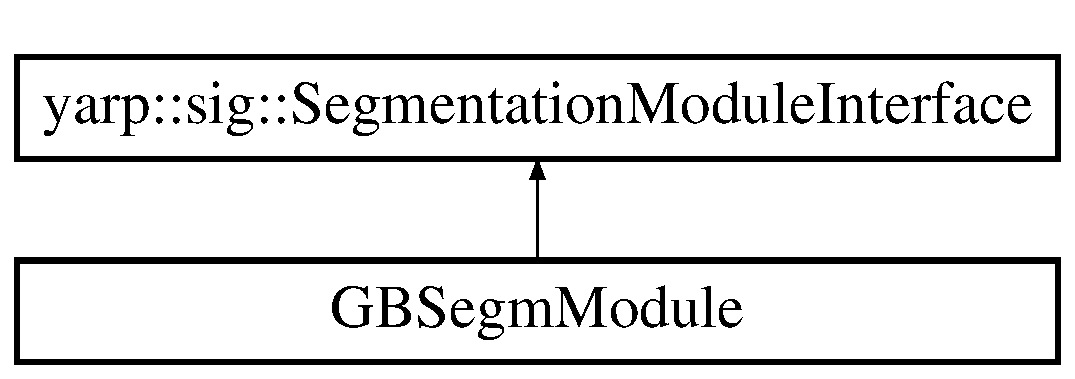
\includegraphics[height=2.000000cm]{classyarp_1_1sig_1_1SegmentationModuleInterface}
\end{center}
\end{figure}
\subsection*{Public Member Functions}
\begin{DoxyCompactItemize}
\item 
virtual void \hyperlink{classyarp_1_1sig_1_1SegmentationModuleInterface_a68f28930df5e930934c0ee56ad1f680c}{set\+\_\+sigma} (const double new\+Value)
\begin{DoxyCompactList}\small\item\em Set sigma (smoothing) parameter for the algorithm. \end{DoxyCompactList}\item 
virtual void \hyperlink{classyarp_1_1sig_1_1SegmentationModuleInterface_a2851eae0226ad68f41cd8b61d8bb1456}{set\+\_\+k} (const double new\+Value)
\begin{DoxyCompactList}\small\item\em Set k (scale factor for boundary-\/detection threshold function) parameter for the algorithm. \end{DoxyCompactList}\item 
virtual void \hyperlink{classyarp_1_1sig_1_1SegmentationModuleInterface_ad9d90ed7e362ae83e2145445a9c4301e}{set\+\_\+min\+Region} (const double new\+Value)
\begin{DoxyCompactList}\small\item\em Set min\+Region parameter for the algorithm, i.\+e., the minimum size of any segmented component. \end{DoxyCompactList}\item 
virtual double \hyperlink{classyarp_1_1sig_1_1SegmentationModuleInterface_a38431f2c63d7da8ebf20adf0ed1da4fe}{get\+\_\+sigma} ()
\begin{DoxyCompactList}\small\item\em Get sigma (smoothing) parameter for the algorithm. \end{DoxyCompactList}\item 
virtual double \hyperlink{classyarp_1_1sig_1_1SegmentationModuleInterface_a91f3d872a48599337d1d2f365ac4c31e}{get\+\_\+k} ()
\begin{DoxyCompactList}\small\item\em Get k (scale factor for boundary-\/detection threshold function) parameter for the algorithm. \end{DoxyCompactList}\item 
virtual double \hyperlink{classyarp_1_1sig_1_1SegmentationModuleInterface_a6c184aeea894f6afcc342c5aa748429d}{get\+\_\+min\+Region} ()
\begin{DoxyCompactList}\small\item\em Get min\+Region parameter for the algorithm, i.\+e., the minimum size of any segmented component. \end{DoxyCompactList}\item 
virtual int32\+\_\+t \hyperlink{classyarp_1_1sig_1_1SegmentationModuleInterface_a3c6b695fbef9e6827e7dd6b4cbbc38fe}{get\+\_\+num\+\_\+components} ()
\begin{DoxyCompactList}\small\item\em Get the number of segmented components that have been detected in the last provided image. \end{DoxyCompactList}\item 
virtual std\+::vector$<$ \hyperlink{classyarp_1_1sig_1_1Pixel}{Pixel} $>$ \hyperlink{classyarp_1_1sig_1_1SegmentationModuleInterface_a9bf0b95fbab216b2284122b0b8a36820}{get\+\_\+component\+\_\+around} (const \hyperlink{classyarp_1_1sig_1_1Pixel}{Pixel} \&obj\+Center)
\begin{DoxyCompactList}\small\item\em Get the list of pixels corresponding to the component to which a given pixel belongs. \end{DoxyCompactList}\item 
virtual bool {\bfseries read} (yarp\+::os\+::\+Connection\+Reader \&connection)\label{classyarp_1_1sig_1_1SegmentationModuleInterface_ae35adf3fde4e4dd6e2dea92b6e396794}

\end{DoxyCompactItemize}


\subsection{Detailed Description}
Interface for module that performs graph-\/based segmentation. 

Definition at line 21 of file Segmentation\+Module\+Interface.\+h.



\subsection{Member Function Documentation}
\index{yarp\+::sig\+::\+Segmentation\+Module\+Interface@{yarp\+::sig\+::\+Segmentation\+Module\+Interface}!get\+\_\+component\+\_\+around@{get\+\_\+component\+\_\+around}}
\index{get\+\_\+component\+\_\+around@{get\+\_\+component\+\_\+around}!yarp\+::sig\+::\+Segmentation\+Module\+Interface@{yarp\+::sig\+::\+Segmentation\+Module\+Interface}}
\subsubsection[{get\+\_\+component\+\_\+around}]{\setlength{\rightskip}{0pt plus 5cm}std\+::vector$<$ {\bf Pixel} $>$ yarp\+::sig\+::\+Segmentation\+Module\+Interface\+::get\+\_\+component\+\_\+around (
\begin{DoxyParamCaption}
\item[{const {\bf Pixel} \&}]{obj\+Center}
\end{DoxyParamCaption}
)\hspace{0.3cm}{\ttfamily [virtual]}}\label{classyarp_1_1sig_1_1SegmentationModuleInterface_a9bf0b95fbab216b2284122b0b8a36820}


Get the list of pixels corresponding to the component to which a given pixel belongs. 


\begin{DoxyParams}{Parameters}
{\em obj\+Center} & a pixel belonging to the region of interest \\
\hline
\end{DoxyParams}
\begin{DoxyReturn}{Returns}
list of pixels belonging to the same component as the input pixels 
\end{DoxyReturn}


Reimplemented in \hyperlink{classGBSegmModule_a0b63c53513e67c4f126e29cf7f28ad53}{G\+B\+Segm\+Module}.



Definition at line 235 of file Segmentation\+Module\+Interface.\+cpp.


\begin{DoxyCode}
235                                                                                           \{
236   std::vector<Pixel>  \_return;
237   SegmentationModuleInterface\_get\_component\_around helper;
238   helper.objCenter = objCenter;
239   \textcolor{keywordflow}{if} (!yarp().canWrite()) \{
240     fprintf(stderr,\textcolor{stringliteral}{"Missing server method '%s'?\(\backslash\)n"},\textcolor{stringliteral}{"std::vector<Pixel> 
       SegmentationModuleInterface::get\_component\_around(const Pixel& objCenter)"});
241   \}
242   \textcolor{keywordtype}{bool} ok = yarp().write(helper,helper);
243   \textcolor{keywordflow}{return} ok?helper.\_return:\_return;
244 \}
\end{DoxyCode}
\index{yarp\+::sig\+::\+Segmentation\+Module\+Interface@{yarp\+::sig\+::\+Segmentation\+Module\+Interface}!get\+\_\+k@{get\+\_\+k}}
\index{get\+\_\+k@{get\+\_\+k}!yarp\+::sig\+::\+Segmentation\+Module\+Interface@{yarp\+::sig\+::\+Segmentation\+Module\+Interface}}
\subsubsection[{get\+\_\+k}]{\setlength{\rightskip}{0pt plus 5cm}double yarp\+::sig\+::\+Segmentation\+Module\+Interface\+::get\+\_\+k (
\begin{DoxyParamCaption}
{}
\end{DoxyParamCaption}
)\hspace{0.3cm}{\ttfamily [virtual]}}\label{classyarp_1_1sig_1_1SegmentationModuleInterface_a91f3d872a48599337d1d2f365ac4c31e}


Get k (scale factor for boundary-\/detection threshold function) parameter for the algorithm. 

\begin{DoxyReturn}{Returns}
current value for k parameter 
\end{DoxyReturn}


Reimplemented in \hyperlink{classGBSegmModule_a44bab99aa7a035e57a185673c040d2f6}{G\+B\+Segm\+Module}.



Definition at line 208 of file Segmentation\+Module\+Interface.\+cpp.


\begin{DoxyCode}
208                                           \{
209   \textcolor{keywordtype}{double} \_return = (double)0;
210   SegmentationModuleInterface\_get\_k helper;
211   \textcolor{keywordflow}{if} (!yarp().canWrite()) \{
212     fprintf(stderr,\textcolor{stringliteral}{"Missing server method '%s'?\(\backslash\)n"},\textcolor{stringliteral}{"double SegmentationModuleInterface::get\_k()"});
213   \}
214   \textcolor{keywordtype}{bool} ok = yarp().write(helper,helper);
215   \textcolor{keywordflow}{return} ok?helper.\_return:\_return;
216 \}
\end{DoxyCode}
\index{yarp\+::sig\+::\+Segmentation\+Module\+Interface@{yarp\+::sig\+::\+Segmentation\+Module\+Interface}!get\+\_\+min\+Region@{get\+\_\+min\+Region}}
\index{get\+\_\+min\+Region@{get\+\_\+min\+Region}!yarp\+::sig\+::\+Segmentation\+Module\+Interface@{yarp\+::sig\+::\+Segmentation\+Module\+Interface}}
\subsubsection[{get\+\_\+min\+Region}]{\setlength{\rightskip}{0pt plus 5cm}double yarp\+::sig\+::\+Segmentation\+Module\+Interface\+::get\+\_\+min\+Region (
\begin{DoxyParamCaption}
{}
\end{DoxyParamCaption}
)\hspace{0.3cm}{\ttfamily [virtual]}}\label{classyarp_1_1sig_1_1SegmentationModuleInterface_a6c184aeea894f6afcc342c5aa748429d}


Get min\+Region parameter for the algorithm, i.\+e., the minimum size of any segmented component. 

\begin{DoxyReturn}{Returns}
current value for min\+Region parameter 
\end{DoxyReturn}


Reimplemented in \hyperlink{classGBSegmModule_a2378b95e60b406a119947aa86b5bb9c4}{G\+B\+Segm\+Module}.



Definition at line 217 of file Segmentation\+Module\+Interface.\+cpp.


\begin{DoxyCode}
217                                                   \{
218   \textcolor{keywordtype}{double} \_return = (double)0;
219   SegmentationModuleInterface\_get\_minRegion helper;
220   \textcolor{keywordflow}{if} (!yarp().canWrite()) \{
221     fprintf(stderr,\textcolor{stringliteral}{"Missing server method '%s'?\(\backslash\)n"},\textcolor{stringliteral}{"double SegmentationModuleInterface::get\_minRegion()"});
222   \}
223   \textcolor{keywordtype}{bool} ok = yarp().write(helper,helper);
224   \textcolor{keywordflow}{return} ok?helper.\_return:\_return;
225 \}
\end{DoxyCode}
\index{yarp\+::sig\+::\+Segmentation\+Module\+Interface@{yarp\+::sig\+::\+Segmentation\+Module\+Interface}!get\+\_\+num\+\_\+components@{get\+\_\+num\+\_\+components}}
\index{get\+\_\+num\+\_\+components@{get\+\_\+num\+\_\+components}!yarp\+::sig\+::\+Segmentation\+Module\+Interface@{yarp\+::sig\+::\+Segmentation\+Module\+Interface}}
\subsubsection[{get\+\_\+num\+\_\+components}]{\setlength{\rightskip}{0pt plus 5cm}int32\+\_\+t yarp\+::sig\+::\+Segmentation\+Module\+Interface\+::get\+\_\+num\+\_\+components (
\begin{DoxyParamCaption}
{}
\end{DoxyParamCaption}
)\hspace{0.3cm}{\ttfamily [virtual]}}\label{classyarp_1_1sig_1_1SegmentationModuleInterface_a3c6b695fbef9e6827e7dd6b4cbbc38fe}


Get the number of segmented components that have been detected in the last provided image. 

\begin{DoxyReturn}{Returns}
number of segmented components 
\end{DoxyReturn}


Reimplemented in \hyperlink{classGBSegmModule_a655ee7c895eed07b07099133b9d8ce68}{G\+B\+Segm\+Module}.



Definition at line 226 of file Segmentation\+Module\+Interface.\+cpp.


\begin{DoxyCode}
226                                                         \{
227   int32\_t \_return = 0;
228   SegmentationModuleInterface\_get\_num\_components helper;
229   \textcolor{keywordflow}{if} (!yarp().canWrite()) \{
230     fprintf(stderr,\textcolor{stringliteral}{"Missing server method '%s'?\(\backslash\)n"},\textcolor{stringliteral}{"int32\_t
       SegmentationModuleInterface::get\_num\_components()"});
231   \}
232   \textcolor{keywordtype}{bool} ok = yarp().write(helper,helper);
233   \textcolor{keywordflow}{return} ok?helper.\_return:\_return;
234 \}
\end{DoxyCode}
\index{yarp\+::sig\+::\+Segmentation\+Module\+Interface@{yarp\+::sig\+::\+Segmentation\+Module\+Interface}!get\+\_\+sigma@{get\+\_\+sigma}}
\index{get\+\_\+sigma@{get\+\_\+sigma}!yarp\+::sig\+::\+Segmentation\+Module\+Interface@{yarp\+::sig\+::\+Segmentation\+Module\+Interface}}
\subsubsection[{get\+\_\+sigma}]{\setlength{\rightskip}{0pt plus 5cm}double yarp\+::sig\+::\+Segmentation\+Module\+Interface\+::get\+\_\+sigma (
\begin{DoxyParamCaption}
{}
\end{DoxyParamCaption}
)\hspace{0.3cm}{\ttfamily [virtual]}}\label{classyarp_1_1sig_1_1SegmentationModuleInterface_a38431f2c63d7da8ebf20adf0ed1da4fe}


Get sigma (smoothing) parameter for the algorithm. 

\begin{DoxyReturn}{Returns}
current value for sigma parameter 
\end{DoxyReturn}


Reimplemented in \hyperlink{classGBSegmModule_ae32ae1b1461e19c3a1b2f429c729ed03}{G\+B\+Segm\+Module}.



Definition at line 199 of file Segmentation\+Module\+Interface.\+cpp.


\begin{DoxyCode}
199                                               \{
200   \textcolor{keywordtype}{double} \_return = (double)0;
201   SegmentationModuleInterface\_get\_sigma helper;
202   \textcolor{keywordflow}{if} (!yarp().canWrite()) \{
203     fprintf(stderr,\textcolor{stringliteral}{"Missing server method '%s'?\(\backslash\)n"},\textcolor{stringliteral}{"double SegmentationModuleInterface::get\_sigma()"});
204   \}
205   \textcolor{keywordtype}{bool} ok = yarp().write(helper,helper);
206   \textcolor{keywordflow}{return} ok?helper.\_return:\_return;
207 \}
\end{DoxyCode}
\index{yarp\+::sig\+::\+Segmentation\+Module\+Interface@{yarp\+::sig\+::\+Segmentation\+Module\+Interface}!set\+\_\+k@{set\+\_\+k}}
\index{set\+\_\+k@{set\+\_\+k}!yarp\+::sig\+::\+Segmentation\+Module\+Interface@{yarp\+::sig\+::\+Segmentation\+Module\+Interface}}
\subsubsection[{set\+\_\+k}]{\setlength{\rightskip}{0pt plus 5cm}void yarp\+::sig\+::\+Segmentation\+Module\+Interface\+::set\+\_\+k (
\begin{DoxyParamCaption}
\item[{const double}]{new\+Value}
\end{DoxyParamCaption}
)\hspace{0.3cm}{\ttfamily [virtual]}}\label{classyarp_1_1sig_1_1SegmentationModuleInterface_a2851eae0226ad68f41cd8b61d8bb1456}


Set k (scale factor for boundary-\/detection threshold function) parameter for the algorithm. 


\begin{DoxyParams}{Parameters}
{\em new\+Value} & new value for k parameter \\
\hline
\end{DoxyParams}


Reimplemented in \hyperlink{classGBSegmModule_a15129913273e221a46c428f697e40575}{G\+B\+Segm\+Module}.



Definition at line 183 of file Segmentation\+Module\+Interface.\+cpp.


\begin{DoxyCode}
183                                                              \{
184   SegmentationModuleInterface\_set\_k helper;
185   helper.newValue = newValue;
186   \textcolor{keywordflow}{if} (!yarp().canWrite()) \{
187     fprintf(stderr,\textcolor{stringliteral}{"Missing server method '%s'?\(\backslash\)n"},\textcolor{stringliteral}{"void SegmentationModuleInterface::set\_k(const double
       newValue)"});
188   \}
189   yarp().write(helper,helper);
190 \}
\end{DoxyCode}
\index{yarp\+::sig\+::\+Segmentation\+Module\+Interface@{yarp\+::sig\+::\+Segmentation\+Module\+Interface}!set\+\_\+min\+Region@{set\+\_\+min\+Region}}
\index{set\+\_\+min\+Region@{set\+\_\+min\+Region}!yarp\+::sig\+::\+Segmentation\+Module\+Interface@{yarp\+::sig\+::\+Segmentation\+Module\+Interface}}
\subsubsection[{set\+\_\+min\+Region}]{\setlength{\rightskip}{0pt plus 5cm}void yarp\+::sig\+::\+Segmentation\+Module\+Interface\+::set\+\_\+min\+Region (
\begin{DoxyParamCaption}
\item[{const double}]{new\+Value}
\end{DoxyParamCaption}
)\hspace{0.3cm}{\ttfamily [virtual]}}\label{classyarp_1_1sig_1_1SegmentationModuleInterface_ad9d90ed7e362ae83e2145445a9c4301e}


Set min\+Region parameter for the algorithm, i.\+e., the minimum size of any segmented component. 


\begin{DoxyParams}{Parameters}
{\em new\+Value} & new value for min\+Region parameter \\
\hline
\end{DoxyParams}


Reimplemented in \hyperlink{classGBSegmModule_ae1c722c9c774cbde4f6bfada3f0826ba}{G\+B\+Segm\+Module}.



Definition at line 191 of file Segmentation\+Module\+Interface.\+cpp.


\begin{DoxyCode}
191                                                                      \{
192   SegmentationModuleInterface\_set\_minRegion helper;
193   helper.newValue = newValue;
194   \textcolor{keywordflow}{if} (!yarp().canWrite()) \{
195     fprintf(stderr,\textcolor{stringliteral}{"Missing server method '%s'?\(\backslash\)n"},\textcolor{stringliteral}{"void SegmentationModuleInterface::set\_minRegion(const
       double newValue)"});
196   \}
197   yarp().write(helper,helper);
198 \}
\end{DoxyCode}
\index{yarp\+::sig\+::\+Segmentation\+Module\+Interface@{yarp\+::sig\+::\+Segmentation\+Module\+Interface}!set\+\_\+sigma@{set\+\_\+sigma}}
\index{set\+\_\+sigma@{set\+\_\+sigma}!yarp\+::sig\+::\+Segmentation\+Module\+Interface@{yarp\+::sig\+::\+Segmentation\+Module\+Interface}}
\subsubsection[{set\+\_\+sigma}]{\setlength{\rightskip}{0pt plus 5cm}void yarp\+::sig\+::\+Segmentation\+Module\+Interface\+::set\+\_\+sigma (
\begin{DoxyParamCaption}
\item[{const double}]{new\+Value}
\end{DoxyParamCaption}
)\hspace{0.3cm}{\ttfamily [virtual]}}\label{classyarp_1_1sig_1_1SegmentationModuleInterface_a68f28930df5e930934c0ee56ad1f680c}


Set sigma (smoothing) parameter for the algorithm. 


\begin{DoxyParams}{Parameters}
{\em new\+Value} & new value for sigma parameter \\
\hline
\end{DoxyParams}


Reimplemented in \hyperlink{classGBSegmModule_a27ffe08d394d321d9f9441423d36ef5e}{G\+B\+Segm\+Module}.



Definition at line 175 of file Segmentation\+Module\+Interface.\+cpp.


\begin{DoxyCode}
175                                                                  \{
176   SegmentationModuleInterface\_set\_sigma helper;
177   helper.newValue = newValue;
178   \textcolor{keywordflow}{if} (!yarp().canWrite()) \{
179     fprintf(stderr,\textcolor{stringliteral}{"Missing server method '%s'?\(\backslash\)n"},\textcolor{stringliteral}{"void SegmentationModuleInterface::set\_sigma(const
       double newValue)"});
180   \}
181   yarp().write(helper,helper);
182 \}
\end{DoxyCode}


The documentation for this class was generated from the following files\+:\begin{DoxyCompactItemize}
\item 
C\+:/dev/icub-\/contrib-\/iit/segmentation/graph\+Based/thrift\+G\+Bseg/include/i\+Cub/segmentation/Segmentation\+Module\+Interface.\+h\item 
C\+:/dev/icub-\/contrib-\/iit/segmentation/graph\+Based/thrift\+G\+Bseg/src/i\+Cub/segmentation/Segmentation\+Module\+Interface.\+cpp\end{DoxyCompactItemize}

%--- End generated contents ---

% Index
\newpage
\phantomsection
\addcontentsline{toc}{chapter}{Index}
\printindex

\end{document}
